\documentclass[aspectratio=169]{beamer}
\usepackage[utf8]{inputenc}
\usepackage{tikz}
\usepackage{amsmath,amsfonts,amsthm,bm, amssymb}
\usepackage{physics}
\usepackage{tabulary}
\usepackage{subcaption}
\usepackage[isbn=false, url=false, doi=false]{biblatex}
\usetheme{metropolis}

\addbibresource{biblio.bib}

\title{Summer project : Hybrid chiral lasers}
\author{Hugo Levy-Falk\\Supervisor : Martin McCall}
\institute{MSc in Optics and Photonics, Imperial College London}
\date{September 2020}

\begin{document}

\begin{frame}
\titlepage
\end{frame}
\begin{frame}{Hybrid chiral lasers}
	{\Huge What does it mean ?}
	\begin{itemize}
		\item Laser $\rightarrow$ O.K.
		\item Hybrid $\rightarrow$ We will come to that later
		\item Chiral ?
	\end{itemize}
	\begin{definition}[Chirality]
		An object is said to be chiral if it is distinguishable from its reflection in a mirror.
	\end{definition}
\end{frame}
\section{Chiral media}
\begin{frame}
	\begin{figure}
		\centering
		\begin{tikzpicture}
			\node [anchor=west] (note) at (-1,6) {\Large Right-handed};
			\node [anchor=west] (note2) at (-1,0.3) {\Large Left-handed};
			\node[anchor=south west,inner sep=0] (image) at (0,0) {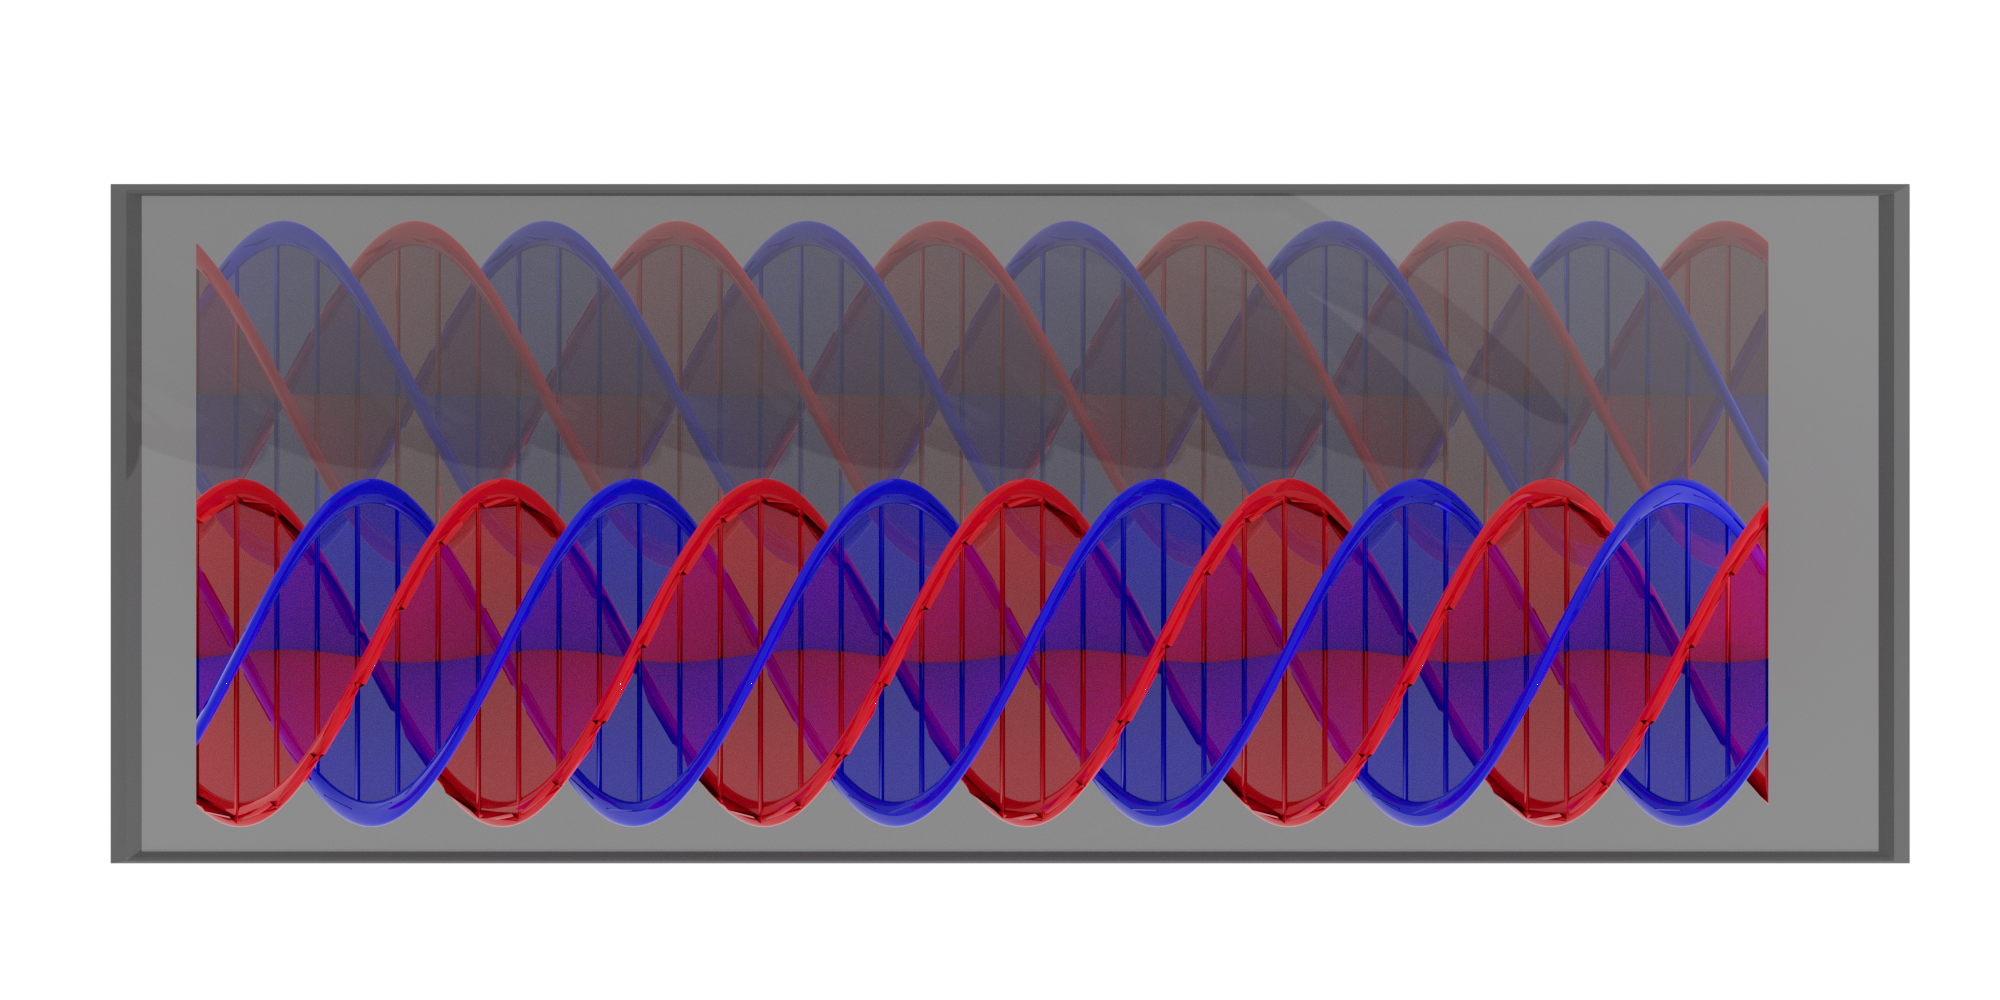
\includegraphics[width=\textwidth]{images/chiral}};
			\begin{scope}[x={(image.south east)},y={(image.north west)}]
				\draw [-latex, ultra thick, red] (note) to[out=0, in=-120] (0.48,0.70);
				\draw [-latex, ultra thick, red] (note2) to[out=0, in=-120] (0.48,0.20);
			\end{scope}
		\end{tikzpicture}
		\caption{A double helix and its reflection in a mirror}
	\end{figure}
\end{frame}

\begin{frame}
	\begin{figure}
		\centering
		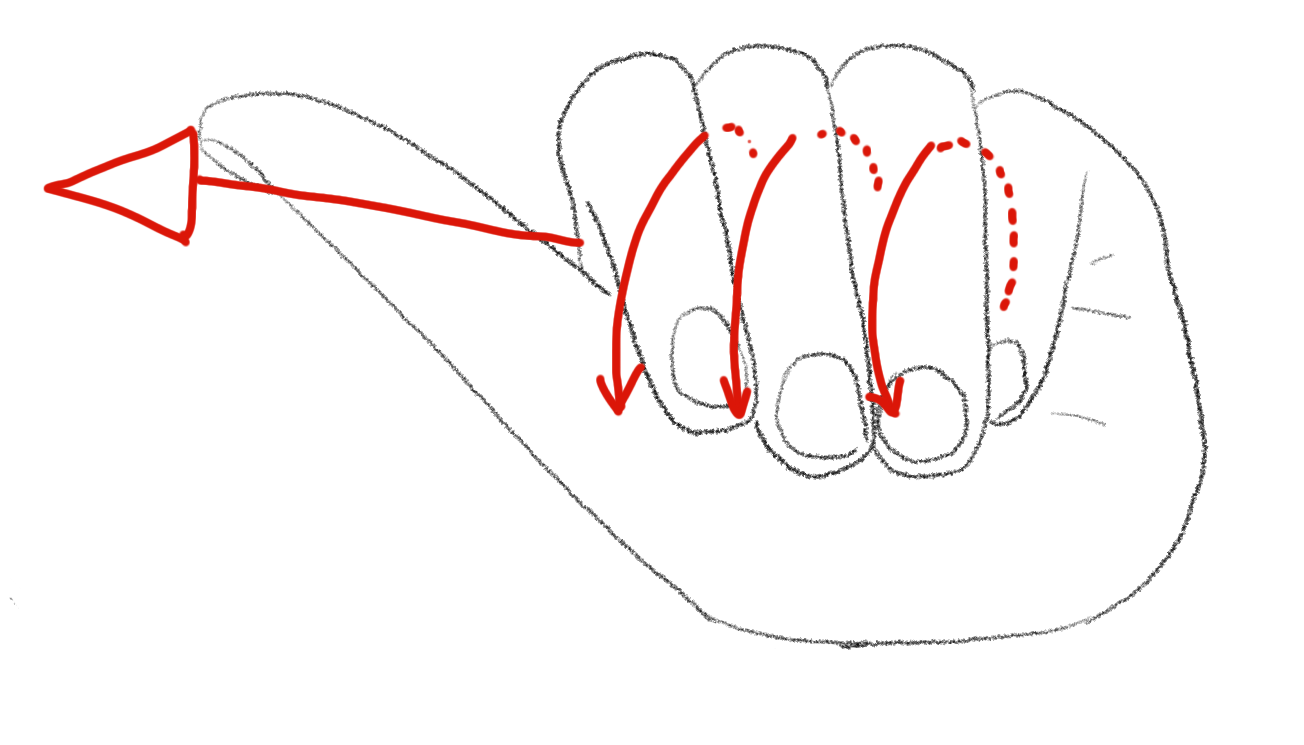
\includegraphics[width=0.7\linewidth]{images/hand}
		\caption{Quick reminder on handedness : left hand}
	\end{figure}
\end{frame}

\begin{frame}{Media studied}
	\begin{columns}
		\begin{column}{0.5\textwidth}
			{\huge A small subset of chiral media}
			\begin{figure}
				\centering
				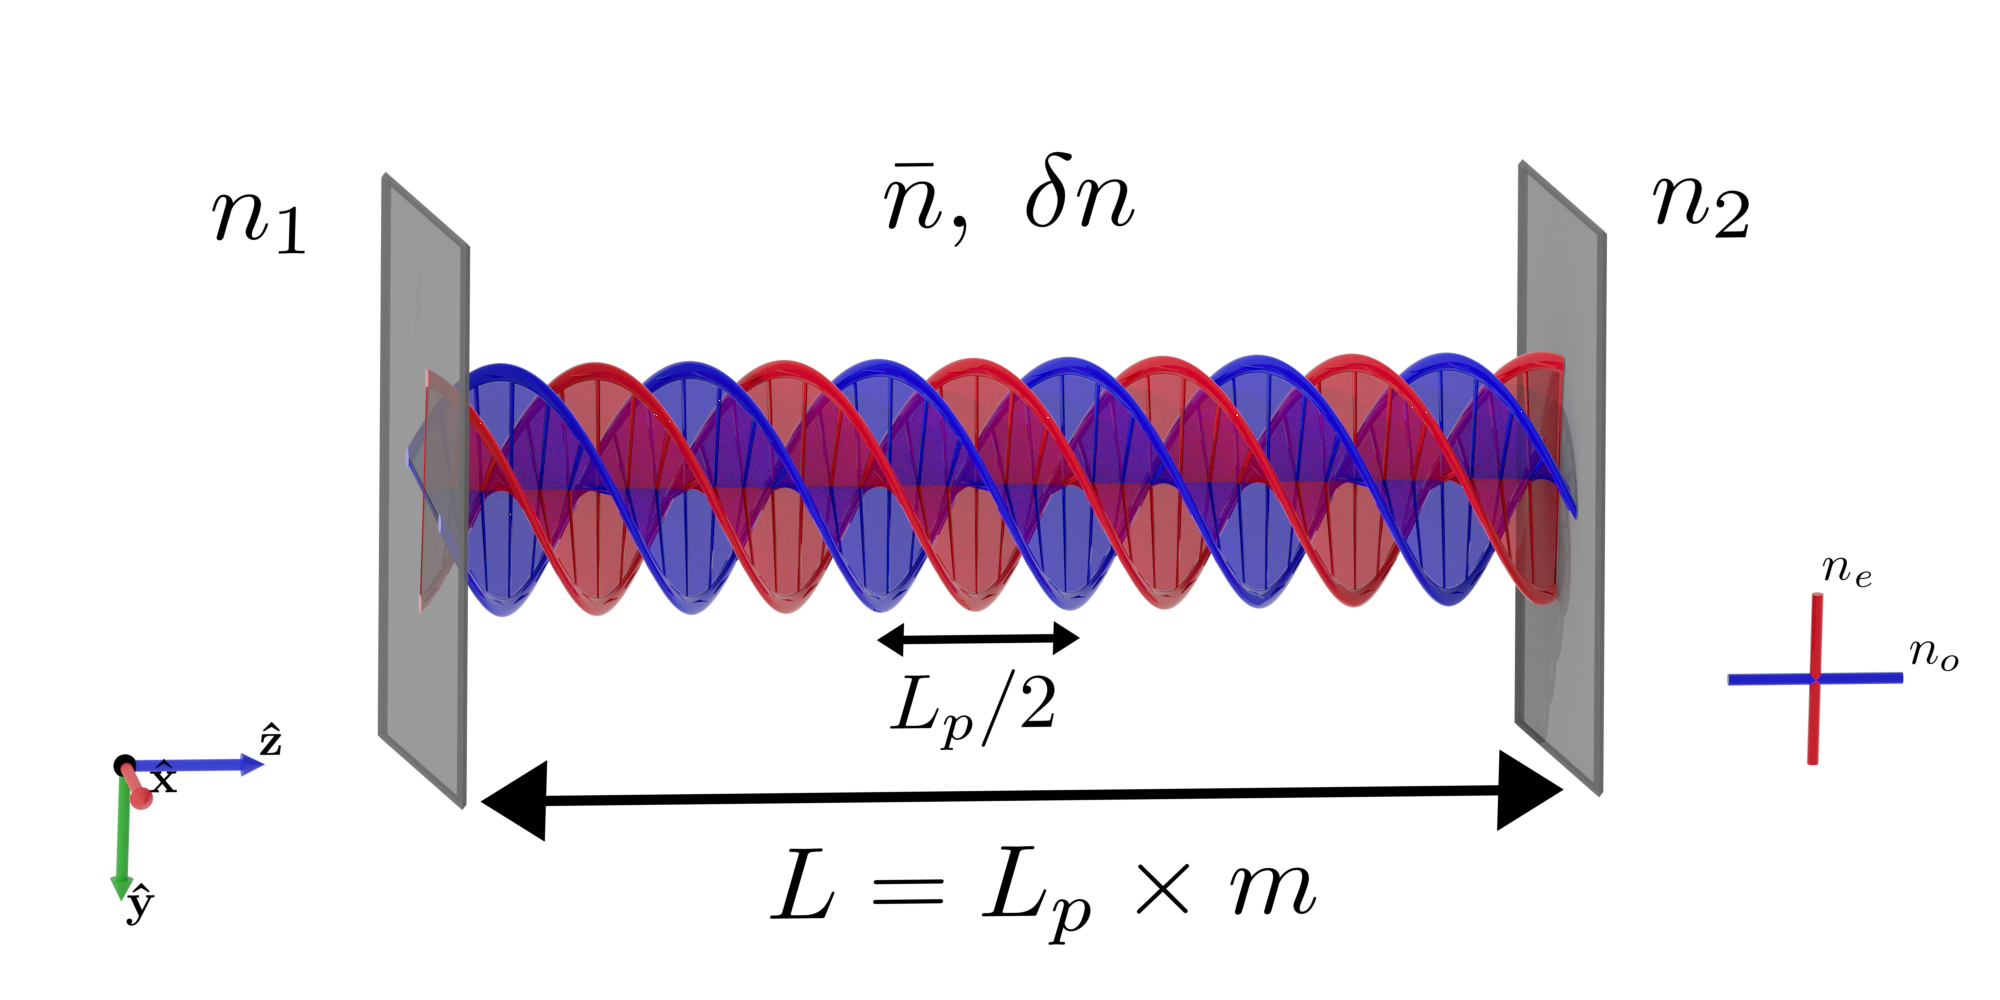
\includegraphics[width=\linewidth]{images/simple_cavity}
				\caption{A slab of chiral medium}
			\end{figure}
		\end{column}
		\begin{column}{0.5\textwidth}
			\begin{equation*}
				\bm{\epsilon} = \begin{pmatrix}\bm{R}^{-1}(z)\cdot\begin{pmatrix}
				\epsilon_a & 0\\
				0 & \epsilon_b\\
				\end{pmatrix}\cdot\bm{R}(z) & \begin{matrix}
				0\\0
				\end{matrix}\\
				\begin{matrix}
				0 & 0
				\end{matrix} & \epsilon_c
				\end{pmatrix}
			\end{equation*}
			\begin{equation*}
				\bm{R}(z) = \begin{pmatrix}
				\cos(pz+\psi) & -\sin(pz+\psi)\\
				\sin(pz+\psi) & \cos(pz+\psi)
				\end{pmatrix}
			\end{equation*}
			\begin{alertblock}{Warning}
				The refractive index does not depend on the position in $(x,y)$ plane.
			\end{alertblock}
		\end{column}
	\end{columns}	
\end{frame}

\section{Studying propagation of light in this medium}

\begin{frame}{Studying propagation of light in this medium}
{\huge Solving Maxwell equations}
\begin{columns}
	\begin{column}{0.5\textwidth}
		\begin{tabulary}{\linewidth}{CC}
			Maxwell-Thomson & Maxwell-Gauss\\
			\(\displaystyle\nabla\cdot\bm{B} = 0\) & \(\displaystyle\nabla\cdot\bm{D}=0\)\\
			Maxwell-Faraday & Maxwell-Ampère\\
			\(\displaystyle\nabla\times\bm{E}=-\pdv{t}\bm{B}\) & \(\displaystyle\nabla\times\bm{H}=\pdv{t}\bm{E}\)\\
			&\\
			\(\displaystyle\bm{D} = \epsilon_0\bm{\epsilon}\bm{E}\) & \(\displaystyle\bm{B} = \mu_0\bm{H}\)
		\end{tabulary}
	\end{column}
	\begin{column}{0.5\textwidth}
		Use auxiliary field $\bm{H}'$ and only study planar component of the field.
		\begin{eqnarray*}
		\bm{H}' &=& \left(\frac{\mu_0}{\epsilon_0}\right)^{1/2}\bm{H}
		\end{eqnarray*}
		\begin{eqnarray*}
		\bm{\hat{z}}\dv{z}\times\bm{E}_\perp &=& ik_0\bm{H}'_\perp\\
		\bm{\hat{z}}\dv{z}\times\bm{H}'_\perp &=& -ik_0\bm{\epsilon}_\perp\cdot\bm{E}_\perp
		\end{eqnarray*}
		\alert{The $\perp$ sign is omitted for convenience.}
	\end{column}
\end{columns}
\end{frame}
\begin{frame}{Studying propagation of light in this medium}
An analytic solution : the Oseen transformation


Rewrite the field from electromagnetic basis to a more convenient basis.
\begin{equation*}
\begin{bmatrix}
\bm{e}(z)\\\bm{h}(z)
\end{bmatrix} = \begin{pmatrix}
\bm{R}^{-1}(z) & \bm{0}\\
\bm{0} & \bm{R}^{-1}(z)
\end{pmatrix}\begin{bmatrix}
\bm{E}(z)\\\bm{H}'(z)
\end{bmatrix}
\end{equation*}
Maxwell's equation are rewritten
\begin{equation*}
\dv{z}\begin{bmatrix}
\bm{e}(z)\\\bm{h}(z)
\end{bmatrix}=i\underbrace{\begin{pmatrix}
	0 & -ip & 0 & k_0\\
	ip & 0 & -k_0 & 0\\
	0 & -k_0\epsilon_b & 0 & -ip\\
	k_0\epsilon_a & 0 & ip & 0\\
	\end{pmatrix}}_{=\bm{G}}\begin{bmatrix}
\bm{e}(z)\\\bm{h}(z)
\end{bmatrix}
\end{equation*}
\end{frame}

\begin{frame}{Studying propagation of light in this medium}
	And this yields a solution.
	\begin{equation*}
	\begin{bmatrix}
	\bm{E}\\\bm{H}'
	\end{bmatrix}_{z=d} = \underbrace{\begin{pmatrix}
		\bm{R}(d) & 0\\0 & \bm{R}(d)
		\end{pmatrix}e^{i\bm{G}d}\begin{pmatrix}
		\bm{R}^{-1}(0) & 0\\0 & \bm{R}^{-1}(0)
		\end{pmatrix}}_{=\bm{M_o}}\begin{bmatrix}
	\bm{E}\\\bm{H}'
	\end{bmatrix}_{z=0}
	\end{equation*}
	Problem solved !
	\alert{Or is it ?}
	\begin{itemize}
		\item Not satisfactory, the transfer matrix is a black-box without any analytic expression of its coefficients
		\item An approximate solution allowing to grasp the underlying dynamics of the cavity is needed.
	\end{itemize}
\end{frame}

\begin{frame}{Studying propagation of light in this medium}
	An approximate solution : the Coupled Waves Theory (CWT)
	\begin{columns}
		\begin{column}{0.5\textwidth}
			The field is decomposed upon the circular basis as:
			\begin{equation*}
			E_{L,R}^\pm = A_{L,R}^\pm e^{\pm ikz}
			\end{equation*}
			\begin{block}{Hypothesis}
				\begin{itemize}
					\item Slow varying envelope approximation;
					\item Neglect field component that are not phase matched.
				\end{itemize}
			\end{block}
		\end{column}
		\begin{column}{0.5\textwidth}
			Maxwell equations become:
			\begin{equation*}
			\dv{z}\bm{A}_{L,R} = \begin{pmatrix}0 & i\kappa e^{-2i\varphi(z)} \\ -i\kappa e^{2i\varphi(z)} & 0\end{pmatrix}\bm{A}_{L,R}
			\end{equation*}
			Where,
			\begin{itemize}
				\item $\kappa = \frac{k_0\delta\epsilon}{2\bar{n}}$
				\item for a right handed medium, $\varphi(z) = \delta kz / 2 - \psi$ and $\delta k = 2(k-p)$;
				\item for a left handed medium, $\varphi(z) = \delta kz / 2 + \psi$ and $\delta k = 2(k+p)$.
			\end{itemize}
		\end{column}
	\end{columns}
\end{frame}

\begin{frame}{Studying propagation of light in this medium}
Solution to CWT equation for \textit{e.g.} right-handed media

\begin{equation*}
\begin{bmatrix}
E_L^+ \\
E_R^+ \\
E_L^- \\
E_R^- \\
\end{bmatrix}_{z=d} = \underbrace{\begin{pmatrix}
	e^{ikd} & 0 & 0 & 0 \\
	0 & \mathcal{P}_R^+ & 0 & \mathcal{Q}_R^+ \\
	0 & 0 & e^{-ikd} & 0 \\
	0 & \mathcal{Q}_R^- & 0 & \mathcal{P}_R^-
	\end{pmatrix}}_{\bm{M_{cwt}}}\begin{bmatrix}
E_L^+ \\
E_R^+ \\
E_L^- \\
E_R^- \\
\end{bmatrix}_{z=0}
\end{equation*}
with
\begin{eqnarray*}
\mathcal{P}_R^\pm &=& \left[\cosh(\Delta d) \pm i \frac{\delta k}{2\Delta}\sinh(\Delta d)\right]e^{\pm ipd}\\
\mathcal{Q}_R^\pm &=& \pm i\frac{\kappa}{\Delta}\sinh(\Delta d) e^{\pm i(pd+2\psi)}
\end{eqnarray*}

\end{frame}

\section{Past results with chiral media}

\begin{frame}{Past results with chiral media}
	\begin{columns}
		\begin{column}{0.5\textwidth}
			\begin{figure}
				\centering
				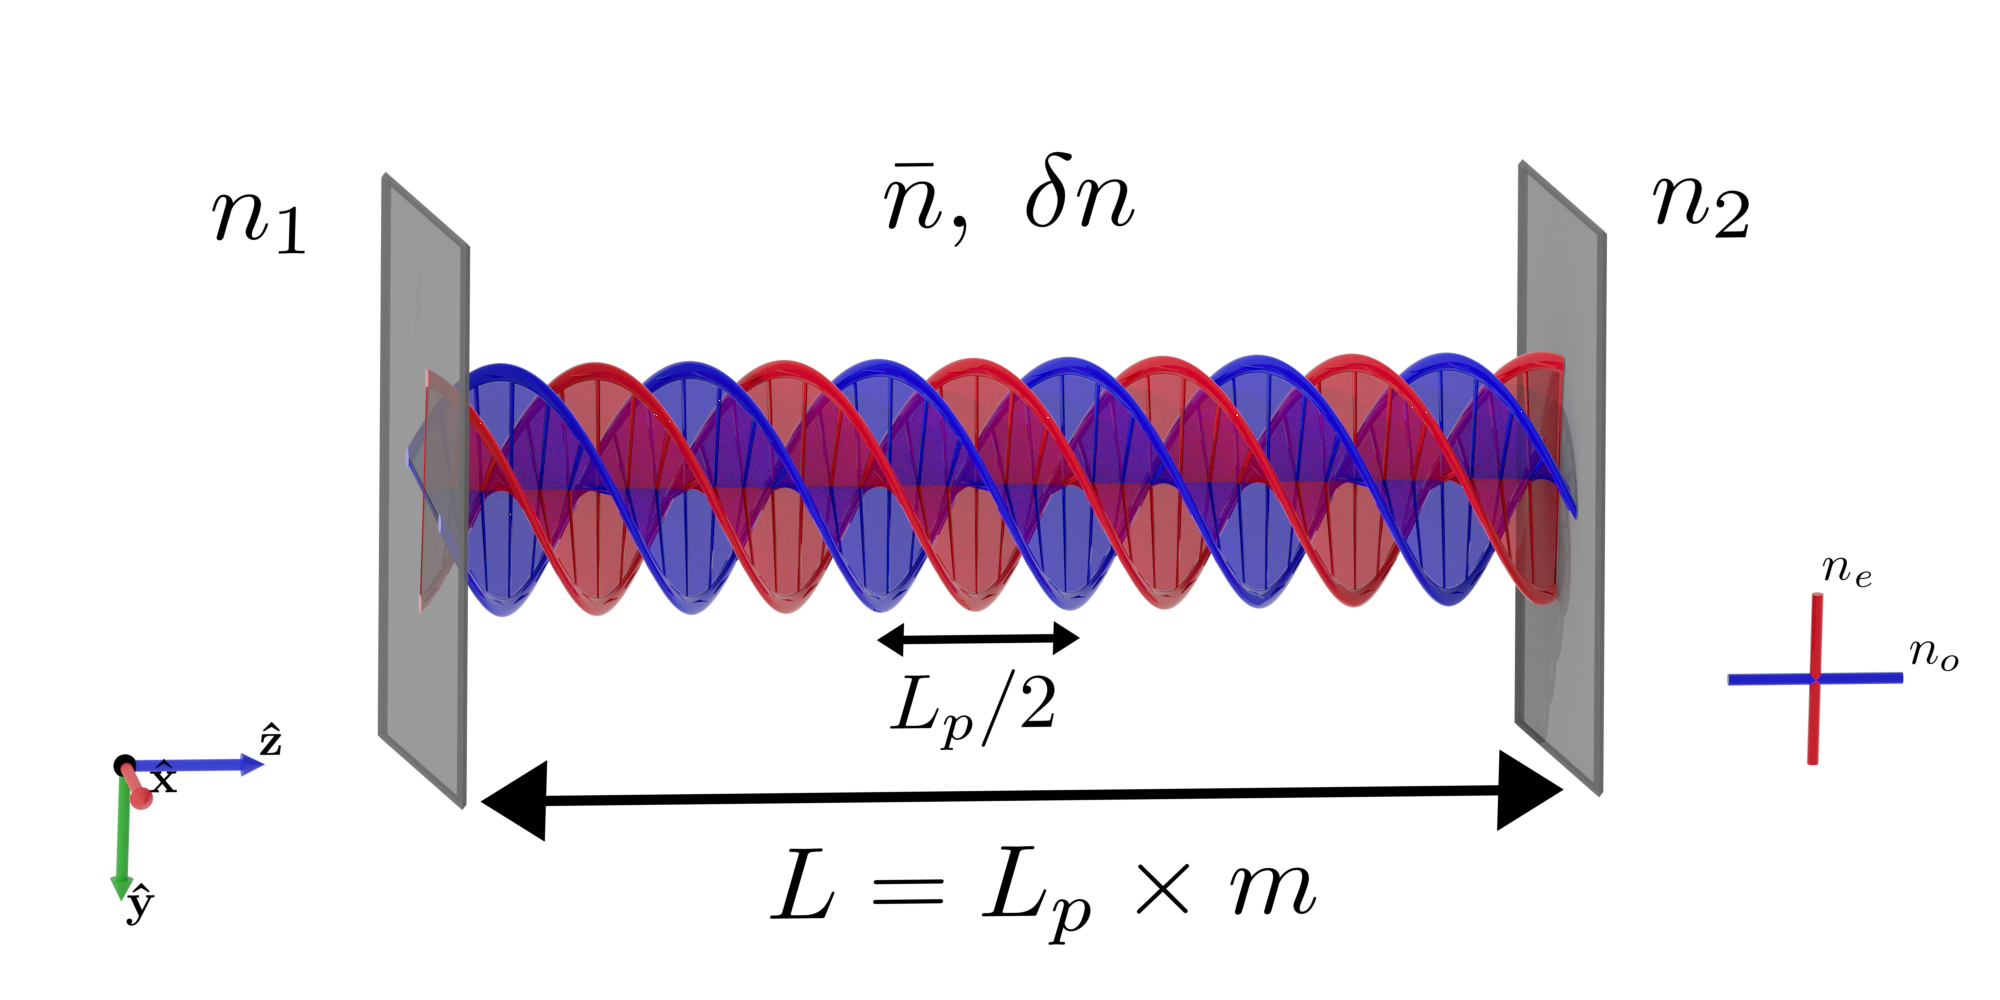
\includegraphics[width=\linewidth]{images/simple_cavity}
				\caption{}
			\end{figure}
			This kind of cavity acts like a Bragg reflector for light polarised with the same handedness as the medium.
		\end{column}
		\begin{column}{0.5\textwidth}
			\begin{figure}
				\centering
				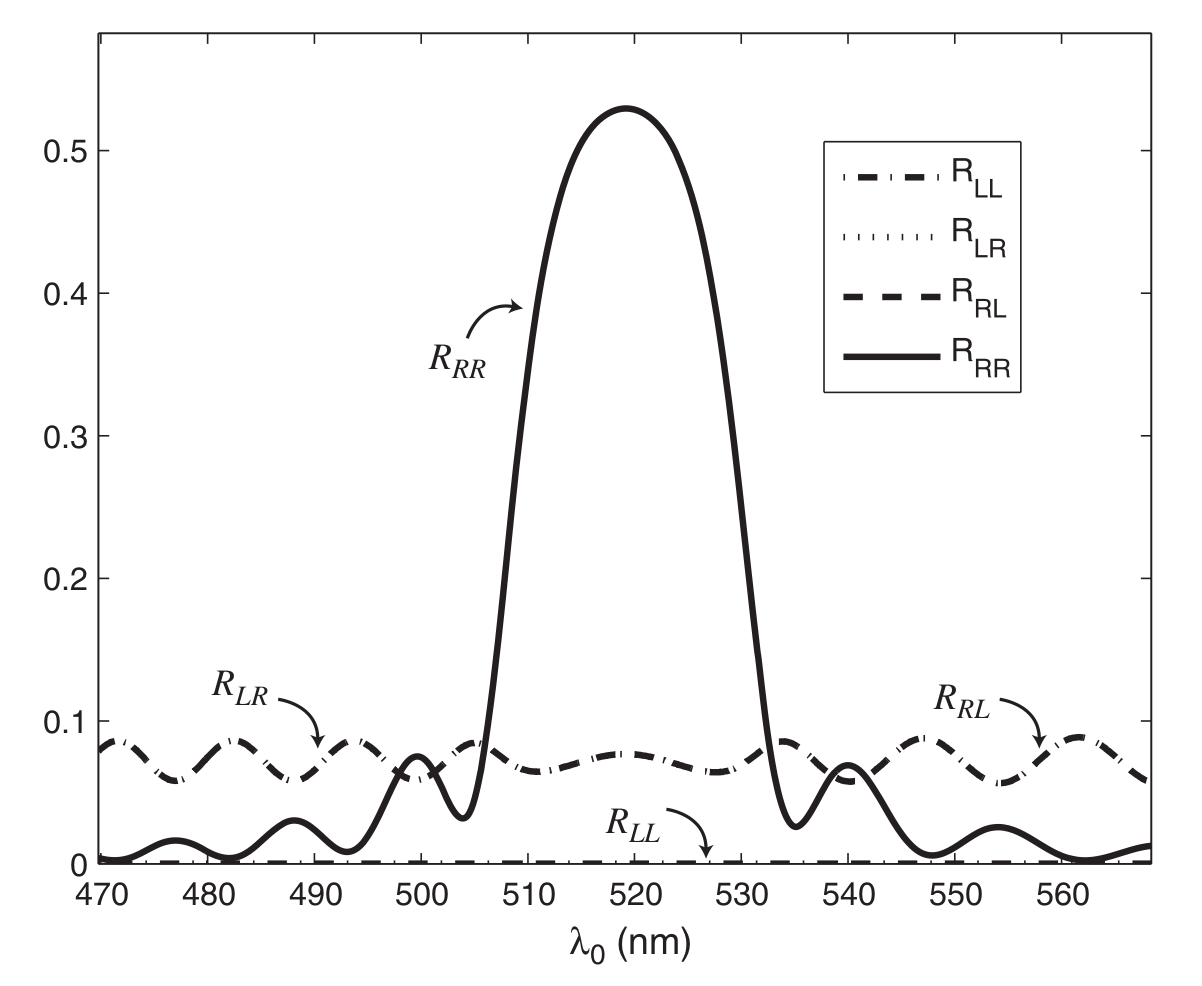
\includegraphics[width=0.8\linewidth]{images/martin_result}
				\caption{Reflectivity of a simulated chiral medium {\tiny \fullcite{mccall_simplified_2009}}}
			\end{figure}
		\end{column}
	\end{columns}
\end{frame}

\begin{frame}{Past results with chiral media}
	\begin{columns}
		\begin{column}{0.5\textwidth}
			This gives complex behaviour when combined to Fresnel reflections at the interfaces. (\fullcite{topf_modes_2014})
		\end{column}
		\begin{column}{0.5\textwidth}
			\begin{figure}
				\centering
				\begin{subfigure}{.49\linewidth}
					\centering
					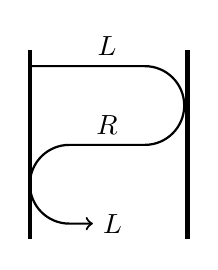
\begin{tikzpicture}
					\draw[ultra thick] (0,-1.2) -- (0,1.2);
					\draw[ultra thick] (2,-1.2) -- (2,1.2);
					\draw[->, thick] (0,1) -- (0.5,1) -- node[above] {$L$} (1.46, 1) arc  (90:-90:0.5) -- node[above] {$R$} (0.5,0) arc (-90:90:-0.5) -- (0.8,-1) node[right] {$L$};
					\end{tikzpicture}
					\caption{}
				\end{subfigure}
				\begin{subfigure}{.49\linewidth}
					\centering
					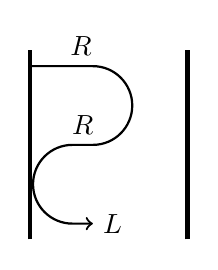
\begin{tikzpicture}
					\draw[ultra thick] (0,-1.2) -- (0,1.2);
					\draw[ultra thick] (2,-1.2) -- (2,1.2);
					\draw[->, thick] (0,1) -- (0.5,1) -- node[above] {$R$} (0.8, 1) arc  (90:-90:0.5) -- node[above] {$R$} (0.54,0) arc (-90:90:-0.5) -- (0.8,-1) node[right] {$L$};
					\end{tikzpicture}
					\caption{}
				\end{subfigure}
				\begin{subfigure}{.49\linewidth}
					\centering
					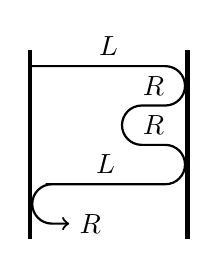
\begin{tikzpicture}
					\draw[ultra thick] (0,-1.2) -- (0,1.2);
					\draw[ultra thick] (2,-1.2) -- (2,1.2);
					\draw[->, thick] (0,1) -- (0.5,1) -- node[above] {$L$} (1.5, 1) -- (1.72,1) arc  (90:-90:0.25) -- node[above] {$R$} (1.42,0.5) arc (-90:90:-0.25) -- node[above]{$R$}(1.72,0) arc  (90:-90:0.25) -- node[above] {$L$} (0.2,-0.5)  -- (0.28,-0.5) arc (-90:90:-0.25) -- (0.5,-1) node[right]{$R$};
					\end{tikzpicture}
					\caption{}
				\end{subfigure}
				\begin{subfigure}{.49\linewidth}
					\centering
					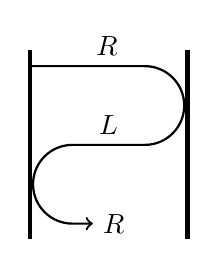
\begin{tikzpicture}
					\draw[ultra thick] (0,-1.2) -- (0,1.2);
					\draw[ultra thick] (2,-1.2) -- (2,1.2);
					\draw[->, thick] (0,1) -- (0.5,1) -- node[above] {$R$} (1.46, 1) arc  (90:-90:0.5) -- node[above] {$L$} (0.54,0) arc (-90:90:-0.5) -- (0.8,-1) node[right] {$R$};
					\end{tikzpicture}
					\caption{}
				\end{subfigure}
			\end{figure}
		\end{column}
	\end{columns}
\end{frame}

\begin{frame}{Past results with chiral media}
	When pumped this creates a relatively un-pure circularly polarised light\footfullcite{topf_modes_2014}.
	\begin{figure}
		\centering
		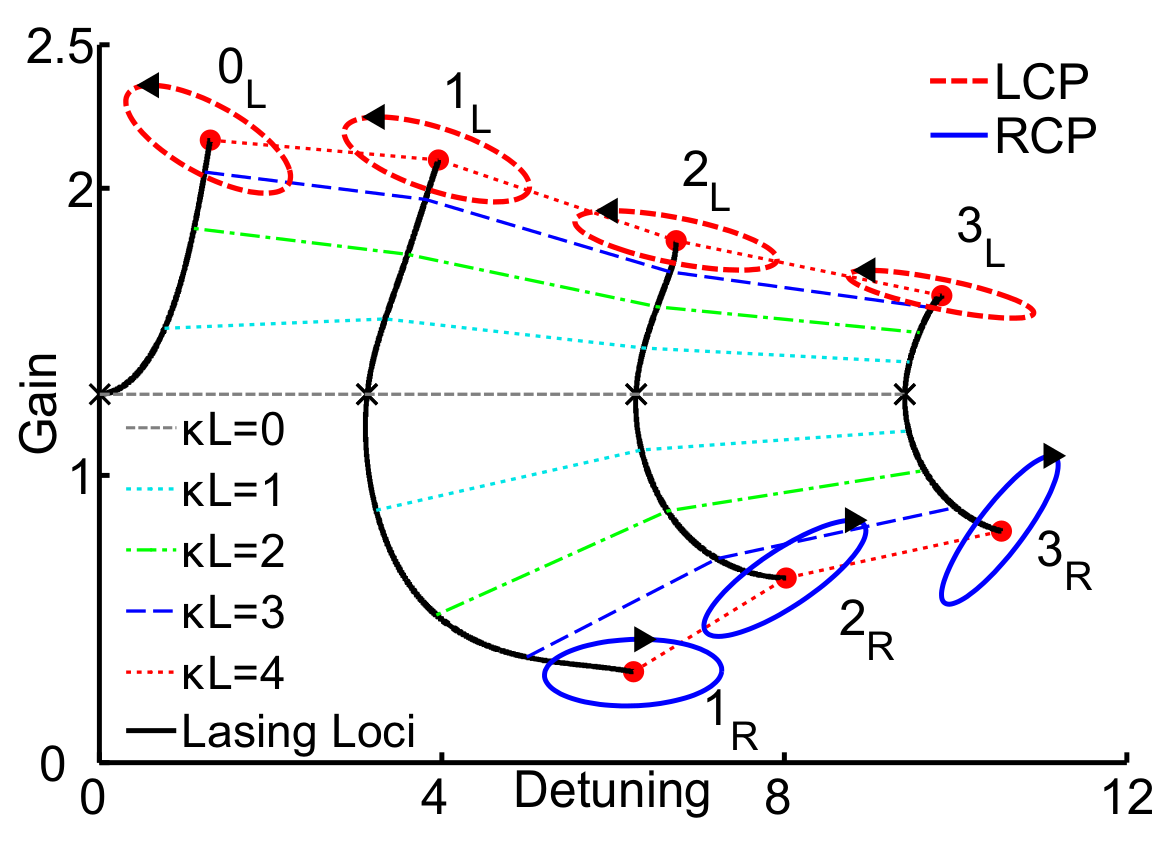
\includegraphics[width=0.4\linewidth]{images/martin_output_mode}
		\caption{}
	\end{figure}
\end{frame}

\section{Objectives}

\begin{frame}{Objectives}
	\begin{figure}
		\centering
		\begin{subfigure}{0.39\linewidth}
			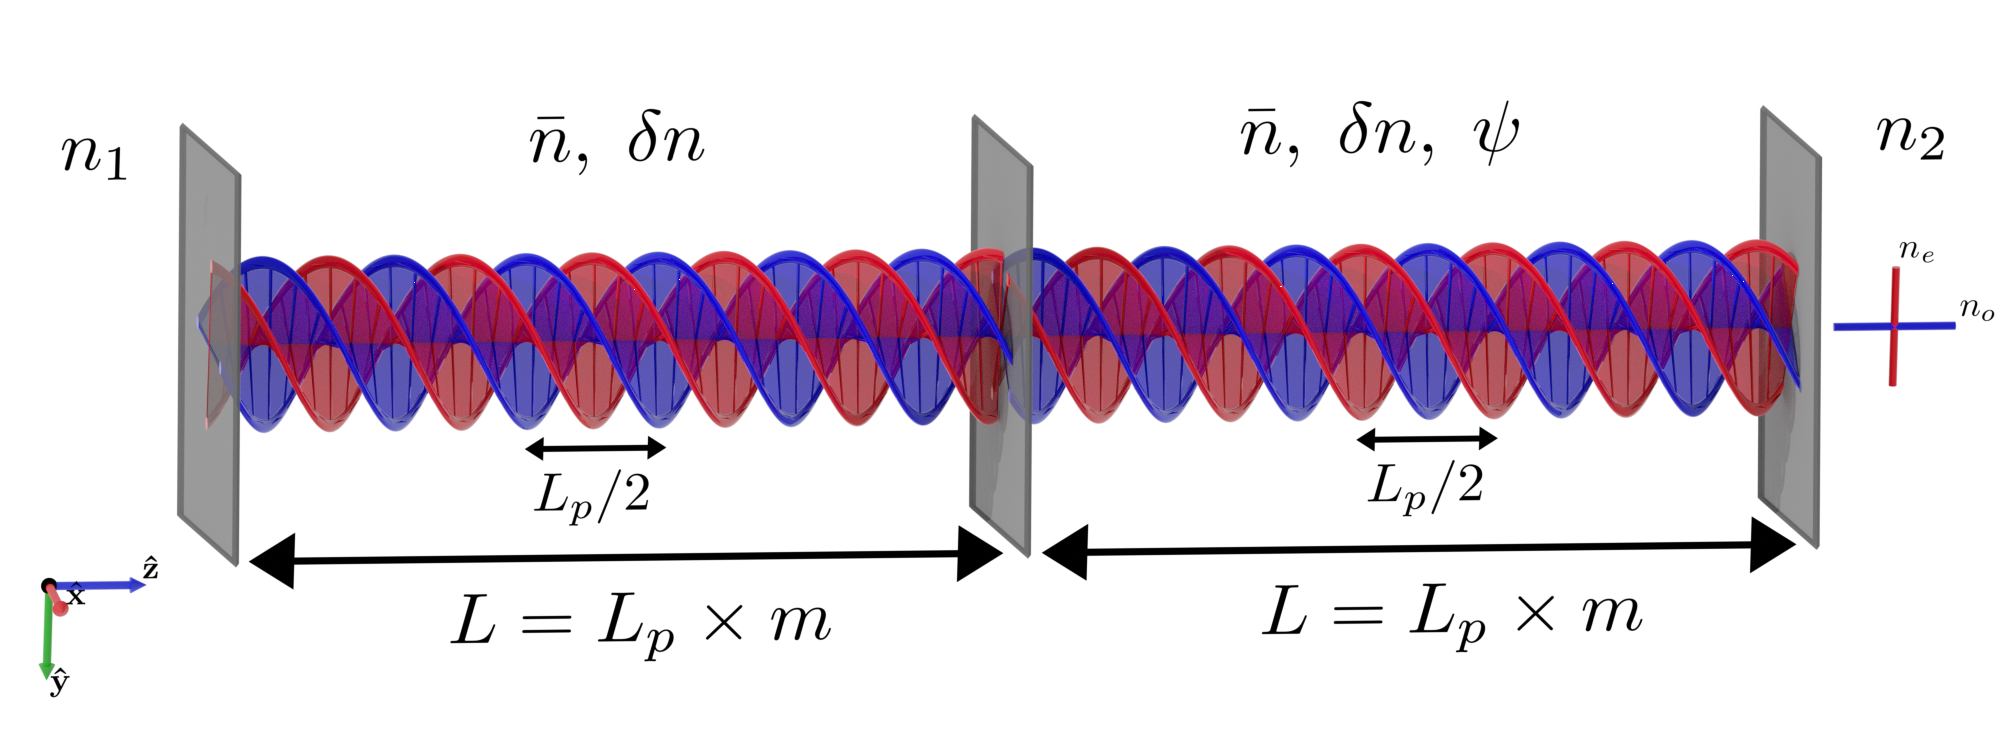
\includegraphics[width=\linewidth]{images/defect.png}
			\caption{Cavity with a defect}
		\end{subfigure}
		\begin{subfigure}{0.60\linewidth}
			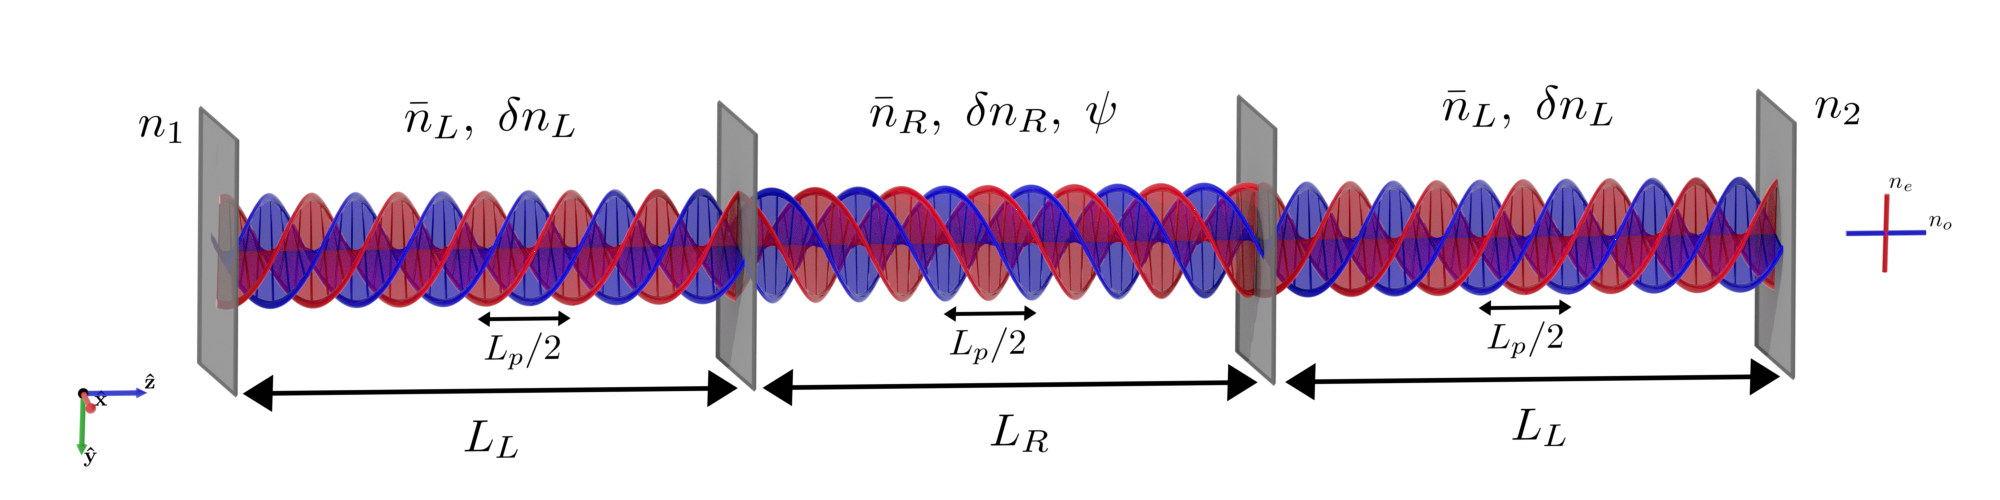
\includegraphics[width=\linewidth]{images/hybrid.png}
			\caption{Hybrid cavity}
		\end{subfigure}
		\begin{subfigure}{\linewidth}
			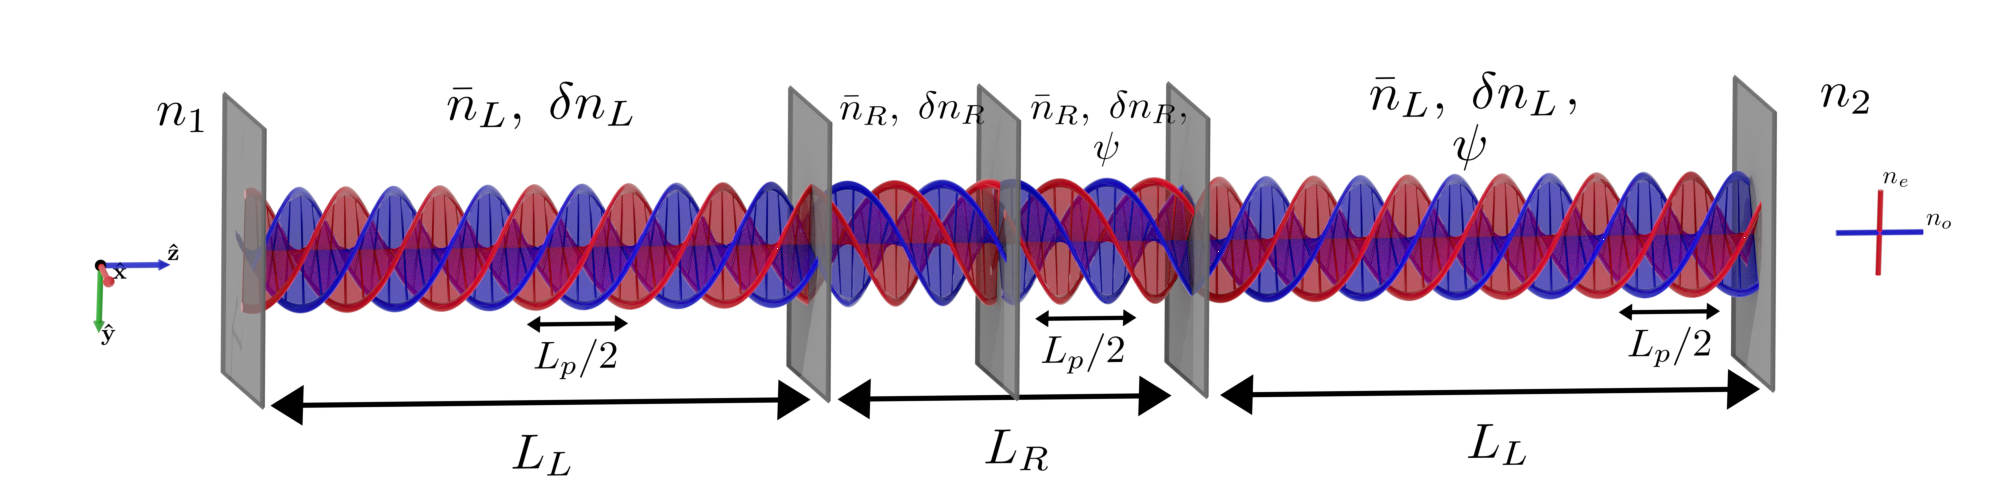
\includegraphics[width=\linewidth]{images/hybrid_defect.png}
			\caption{Hybrid defect cavity}
		\end{subfigure}
		\caption{}
	\end{figure}
\end{frame}

\section{Method}

\begin{frame}{Method}
	\alert{How to calculate reflectivities ?}
	
	\begin{columns}
		\begin{column}{0.5\textwidth}
			Partial inverse of a matrix allows determining the reflection and transmission matrices
			\begin{equation*}
			\begin{bmatrix}
			E_a^+ \\
			E_b^+ \\
			E_a^- \\
			E_b^- \\
			\end{bmatrix}_{1} = \begin{pmatrix}
			\bm{M_{11}} & \bm{M_{12}}\\
			\bm{M_{21}} & \bm{M_{22}}\\
			\end{pmatrix}\begin{bmatrix}
			E_a^+ \\
			E_b^+ \\
			E_a^- \\
			E_b^- \\
			\end{bmatrix}_{0}
			\end{equation*}
		\end{column}
		\begin{column}{0.5\textwidth}
			As 
			\begin{eqnarray*}
				\begin{pmatrix}
					t_{aa} & t_{ab} \\
					t_{ba} & t_{bb}
				\end{pmatrix} &=& \bm{M_{11}} - \bm{M_{12}}\bm{M_{22}}^{-1}\bm{M_{21}}\\
				\begin{pmatrix}
					r_{aa} & r_{ab} \\
					r_{ba} & r_{bb}
				\end{pmatrix} &=& -\bm{M_{22}}^{-1}\bm{M_{21}}
			\end{eqnarray*}
		\end{column}
	\end{columns}
\end{frame}

\begin{frame}{Method}
	\alert{How to characterise laser action ?}
	\begin{columns}
		\begin{column}{0.5\textwidth}
			For a cavity of length $L$.
		\begin{equation*}
		\begin{bmatrix}
		E_a^+ \\
		E_b^+ \\
		0 \\
		0 \\
		\end{bmatrix}_{L^+} = \begin{pmatrix}
		\bm{M_{11}} & \bm{M_{12}}\\
		\bm{M_{21}} & \bm{M_{22}}\\
		\end{pmatrix}\begin{bmatrix}
		0 \\
		0 \\
		E_a^- \\
		E_b^- \\
		\end{bmatrix}_{0^-}
		\end{equation*}
		\end{column}
		\begin{column}{0.5\textwidth}
			That means
			\begin{equation*}
				\abs{\bm{M_{22}}} = 0
			\end{equation*}
			The output mode can be retrieved we the eigen-vector in the kernel of $\bm{M_{22}}$.
		\end{column}
	\end{columns}
\end{frame}
\section{Results}

\begin{frame}{Results : Defect cavity}
	\begin{figure}
		\centering
		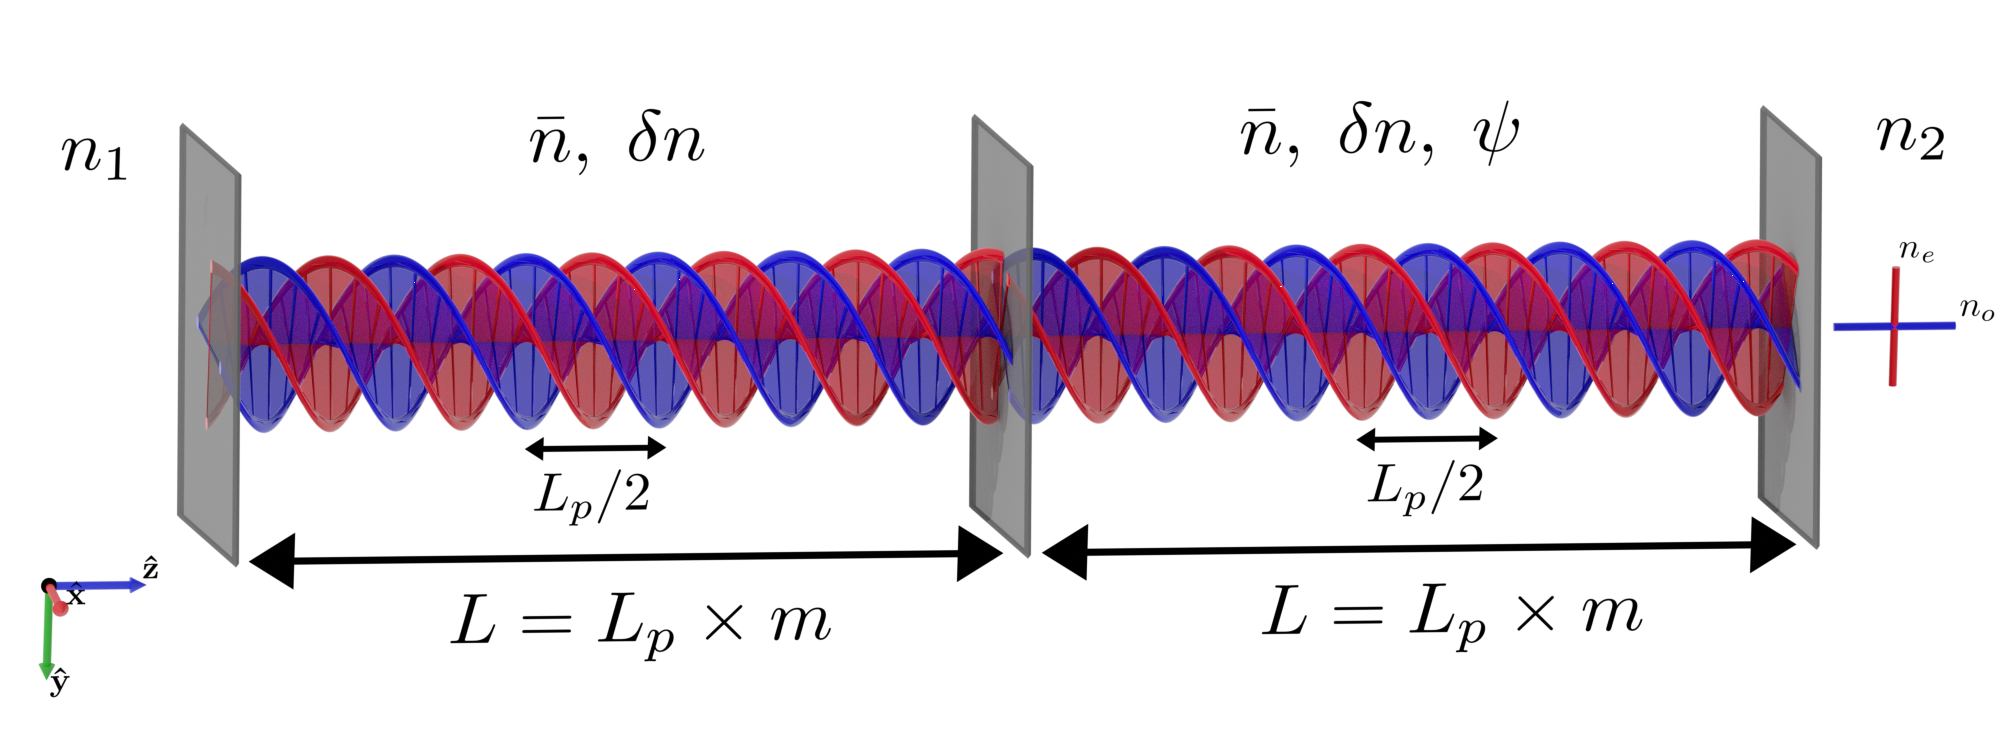
\includegraphics[width=\linewidth]{images/defect.png}
		\caption{Cavity with a defect}
	\end{figure}
\end{frame}
\begin{frame}{Results : Defect cavity}
	\begin{figure}
		\begin{subfigure}{0.32\textwidth}
			\centering
			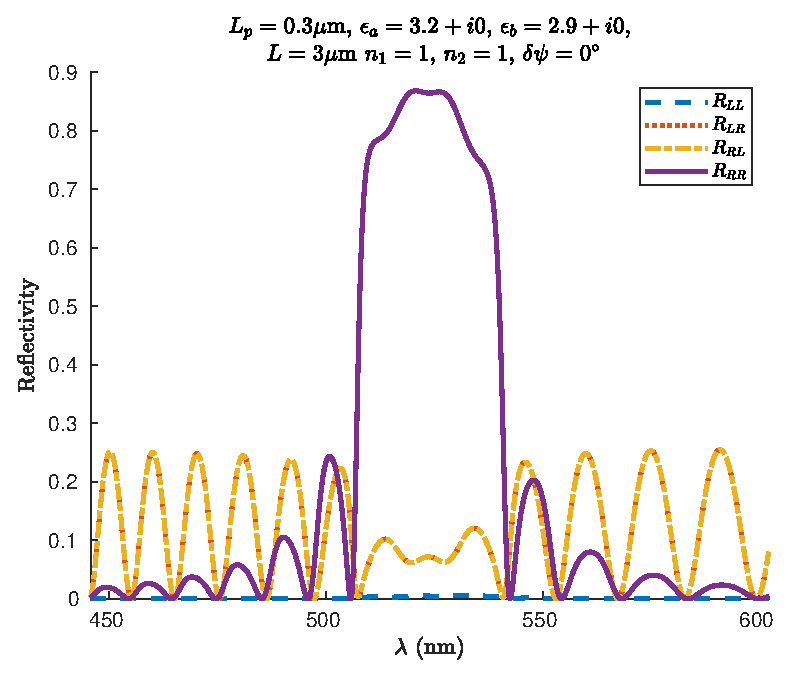
\includegraphics[width=\linewidth]{plots/defect/no_defect/oseen_reflection}
			\caption{Cavity without a defect}
		\end{subfigure}
		\begin{subfigure}{0.32\textwidth}
			\centering
			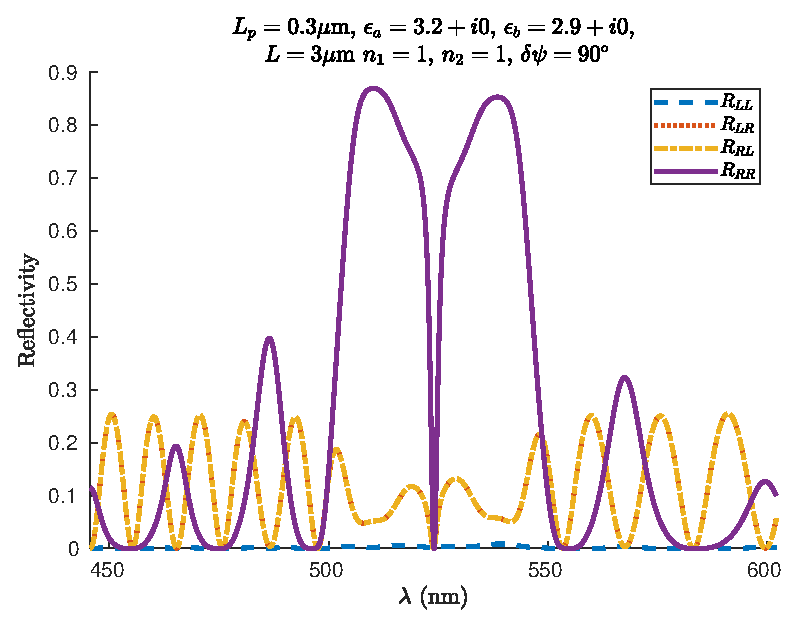
\includegraphics[width=\linewidth]{plots/defect/reflectivity/oseen_reflection}
			\caption{Cavity with a $\frac{\pi}{2}$ defect}
		\end{subfigure}
		\begin{subfigure}{0.32\textwidth}
			\centering
			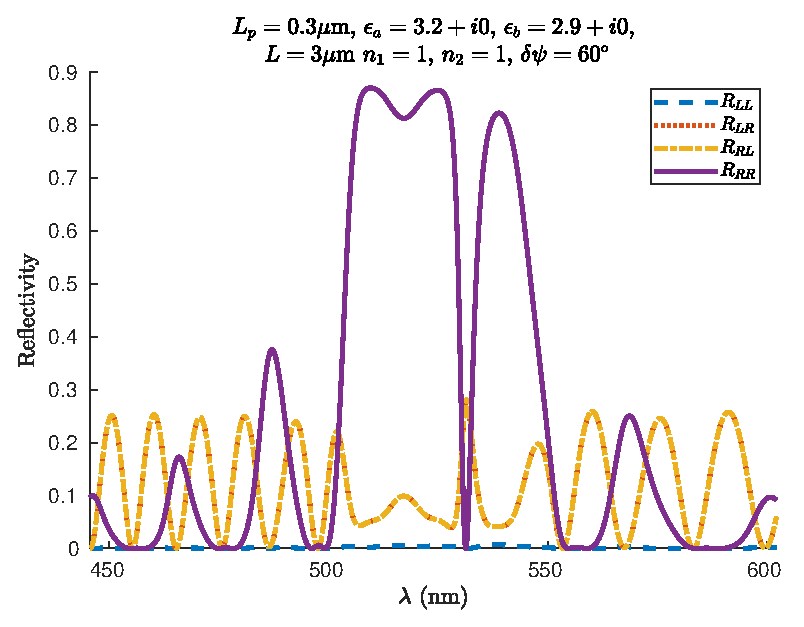
\includegraphics[width=\linewidth]{plots/defect/reflectivity_other_defect/oseen_reflection}
			\caption{Cavity with a $\frac{\pi}{3}$ defect}
		\end{subfigure}
	\end{figure}
\end{frame}

\begin{frame}{Results : Defect cavity}
	\begin{figure}
		\centering
		\begin{subfigure}{0.49\linewidth}
			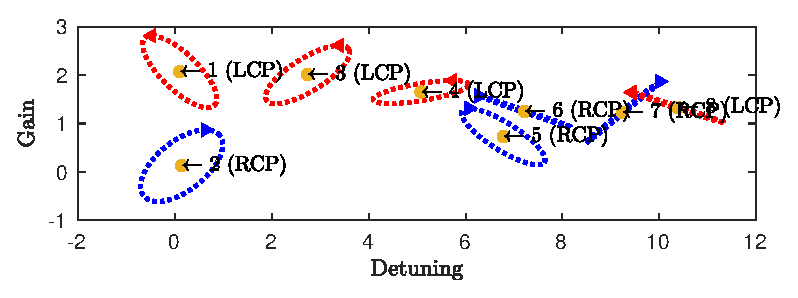
\includegraphics[width=\linewidth]{plots/defect/modes_found}
			\caption{Modes found for $\pi/2$ defect}
		\end{subfigure}
		\begin{subfigure}{0.49\linewidth}
			\centering
			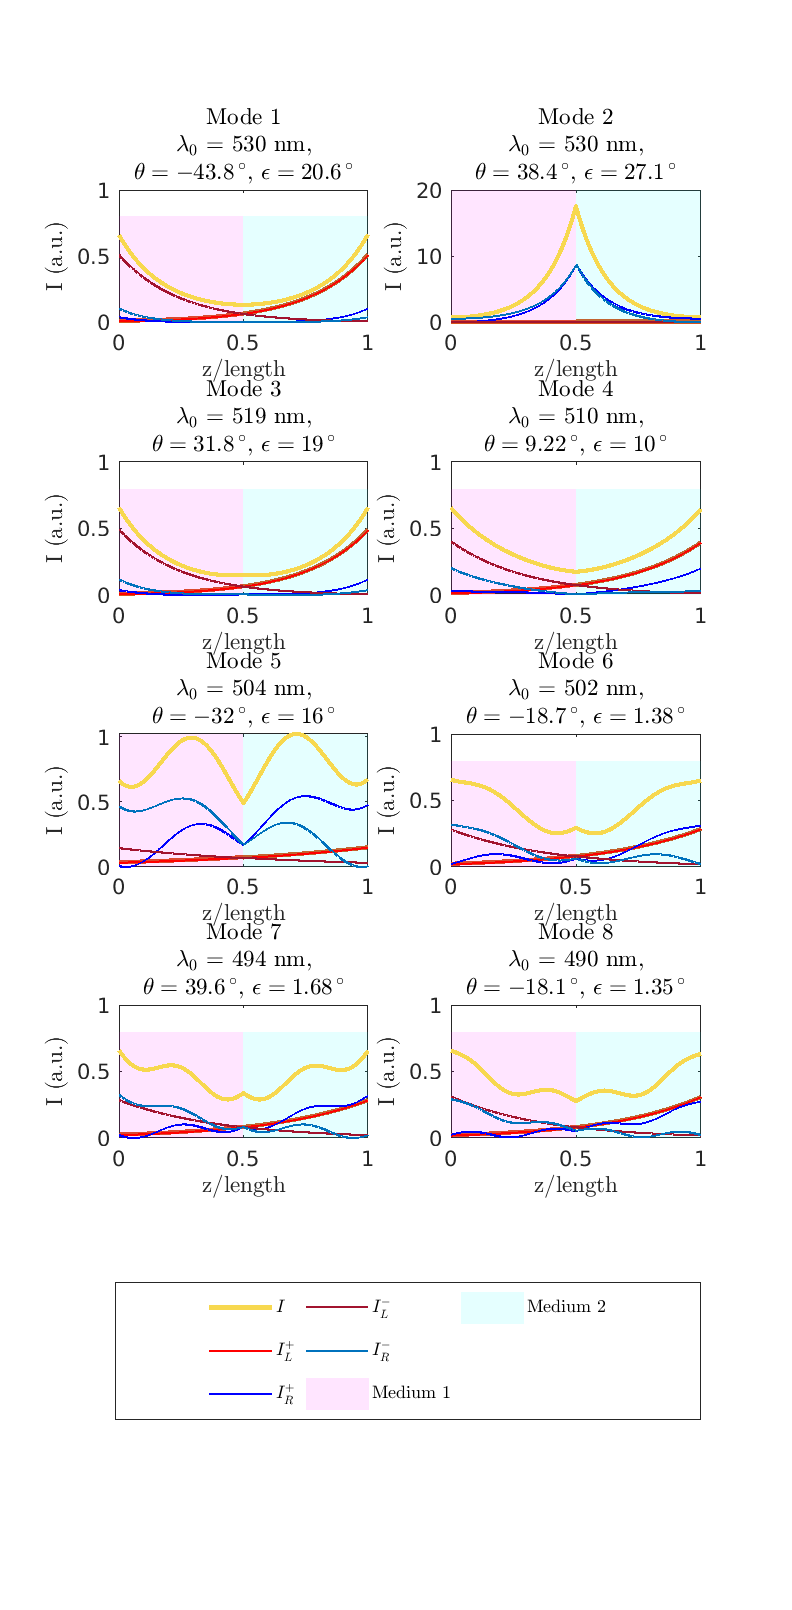
\includegraphics[height=\textheight]{plots/defect/intensity_distribution}
		\end{subfigure}
	\end{figure}
\end{frame}

\begin{frame}{Results : Defect cavity}
	\begin{figure}
		\centering
		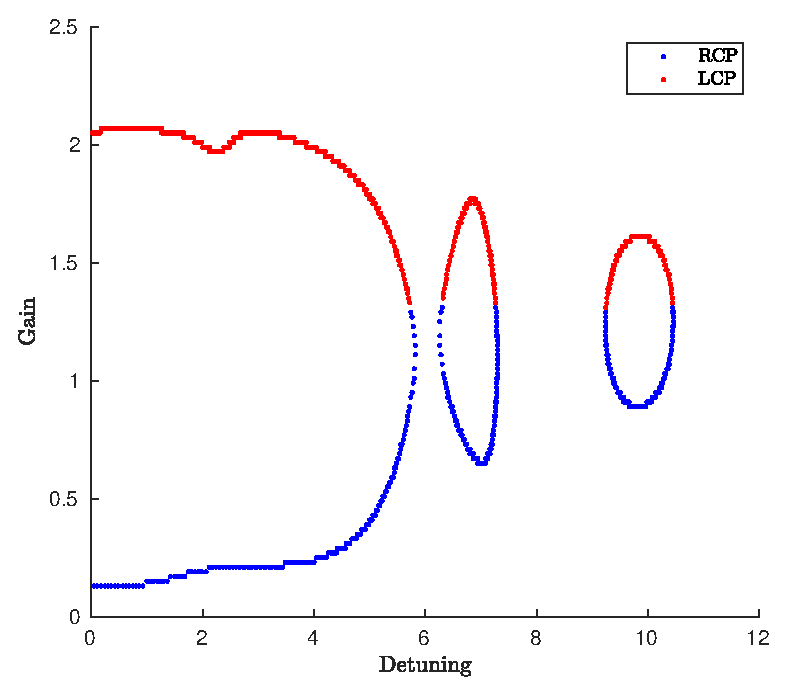
\includegraphics[width=0.5\linewidth]{plots/defect/tuning}
		\caption{Tuning of the cavity}
	\end{figure}
\end{frame}

\begin{frame}{Results : Hybrid cavity}
\begin{figure}
	\centering
	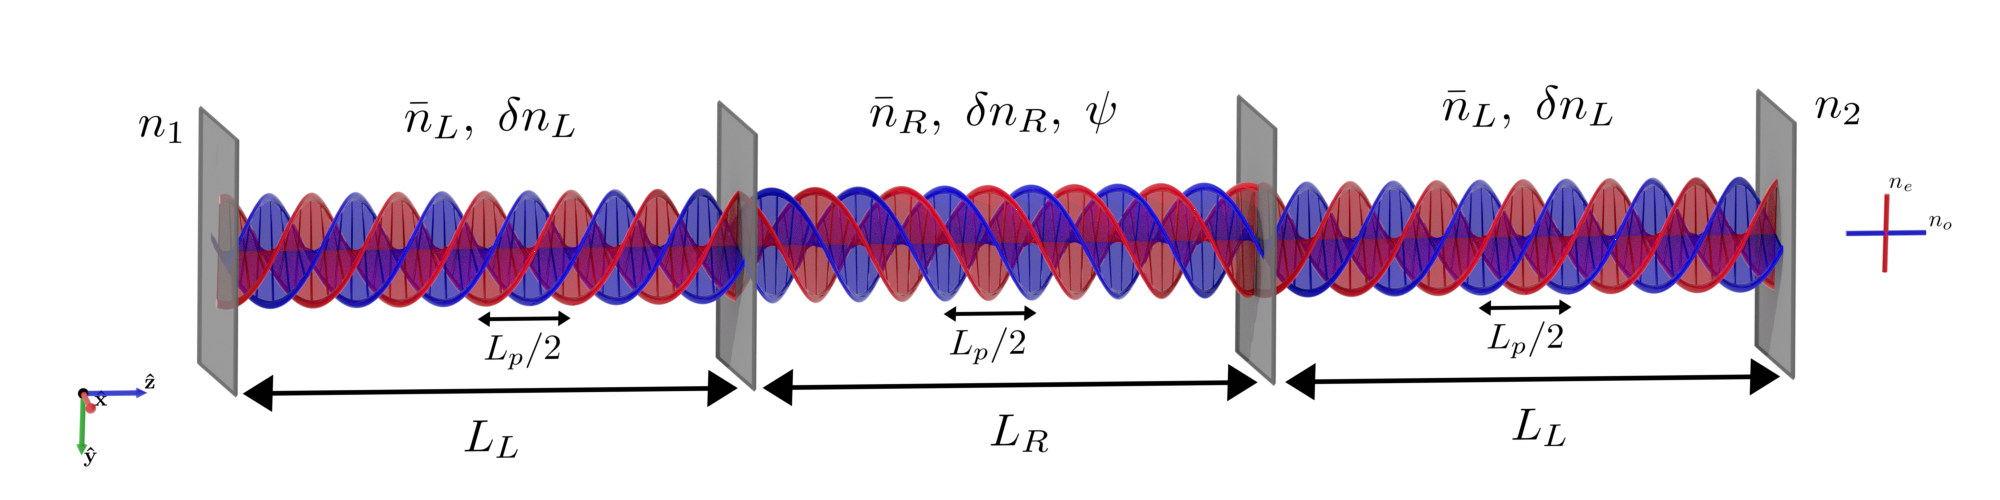
\includegraphics[width=\linewidth]{images/hybrid.png}
	\caption{Hybrid cavity}
\end{figure}
\end{frame}

\begin{frame}{Results : Hybrid cavity}
	\begin{figure}
		\centering
		\begin{subfigure}{0.49\textwidth}
			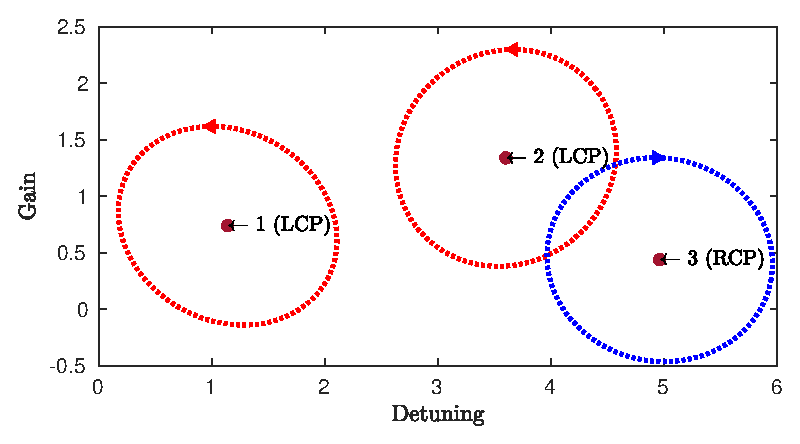
\includegraphics[width=\linewidth]{plots/hybrid/modes_found}
		\end{subfigure}
		\begin{subfigure}{0.49\textwidth}
			\centering
			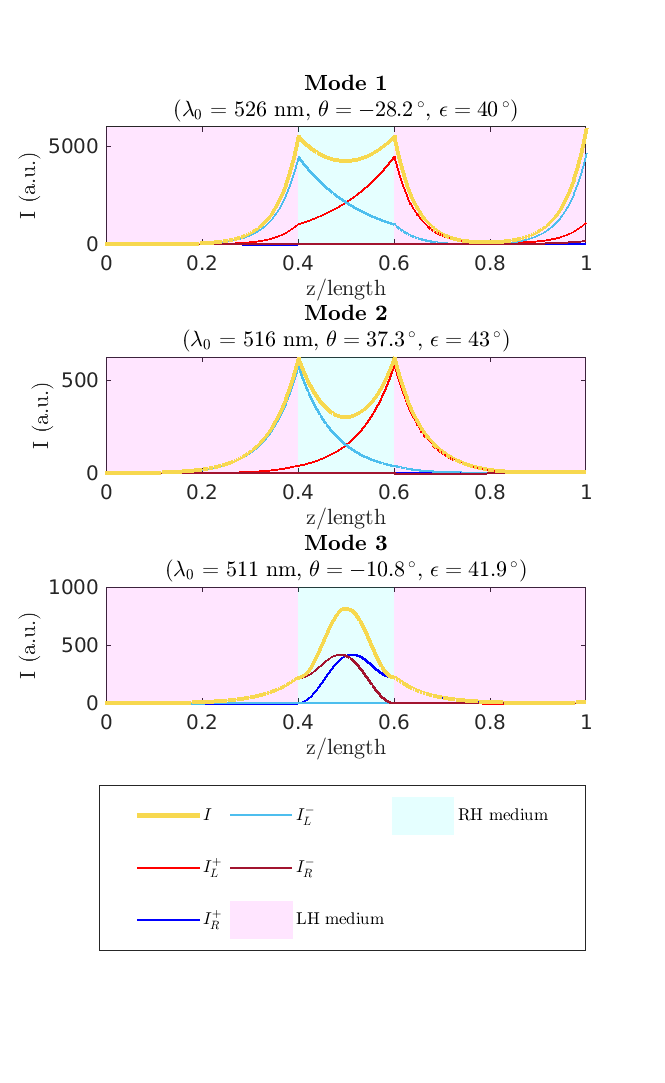
\includegraphics[height=0.8\textheight]{plots/hybrid/intensity_distribution}
		\end{subfigure}	
	\end{figure}
\end{frame}

\begin{frame}{Results : Hybrid cavity}
	\begin{figure}
		\centering
		\begin{subfigure}{0.48\linewidth}
			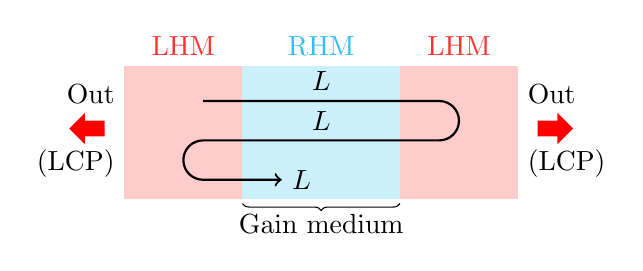
\begin{tikzpicture}
			\fill[red!20] (-1.5,1.2) -- (0,1.2) -- (0,-0.5) -- (-1.5,-0.5) -- cycle;
			\fill[red!20] (2,1.2) -- (3.5,1.2) -- (3.5,-0.5) -- (2,-0.5) -- cycle;
			\fill[cyan!20] (0,1.2) -- (2,1.2) -- (2,-0.5) -- (0,-0.5) -- cycle;
			\draw[red!80] (-0.75,1.2)node [above] {LHM} ;
			\draw[red!80] (2.75,1.2)node [above] {LHM} ;
			\draw[cyan!80] (1,1.2)node [above] {RHM} ;
			
			\draw[->, thick] (-0.5,0.75) -- node[above] {$L$} (2.5,0.75) arc  (90:-90:0.25) -- node[above] {$L$} (-0.5,0.25) arc (90:270:0.25) -- (0.5,-0.25) node[right] {$L$};
			\draw[decoration={brace,mirror,raise=1.5pt},decorate] (0,-0.5) -- node[below=2pt] {Gain medium} (2,-0.5);
			
			\fill[red] (3.75,0.5) -- (4,0.5) -- (4,0.6) -- (4.2,0.4) -- (4,0.2) -- (4,0.3) -- (3.75,0.3) -- cycle;
			\node[above right] at (3.5,0.6) {Out};
			\node[below right] at (3.5,0.25) {(LCP)};			
			
			\fill[red] (-1.75,0.5) -- (-2,0.5) -- (-2,0.6) -- (-2.2,0.4) -- (-2,0.2) -- (-2,0.3) -- (-1.75,0.3) -- cycle;
			\node[above left] at (-1.5,0.6) {Out};
			\node[below left] at (-1.5,0.25) {(LCP)};
			
			\end{tikzpicture}
			\caption{}
			\label{fig:hybrid:mechanism_lh}
		\end{subfigure}
		\begin{subfigure}{0.48\linewidth}
			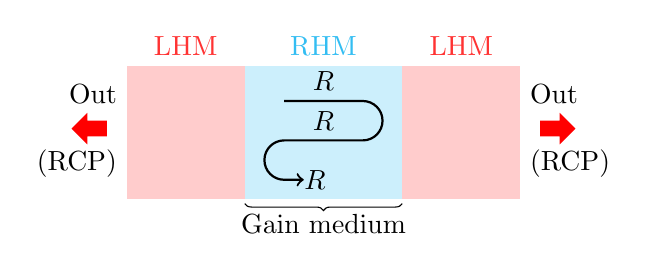
\begin{tikzpicture}
			\fill[red!20] (-1.5,1.2) -- (0,1.2) -- (0,-0.5) -- (-1.5,-0.5) -- cycle;
			\fill[red!20] (2,1.2) -- (3.5,1.2) -- (3.5,-0.5) -- (2,-0.5) -- cycle;
			\fill[cyan!20] (0,1.2) -- (2,1.2) -- (2,-0.5) -- (0,-0.5) -- cycle;
			\draw[red!80] (-0.75,1.2)node [above] {LHM} ;
			\draw[red!80] (2.75,1.2)node [above] {LHM} ;
			\draw[cyan!80] (1,1.2)node [above] {RHM} ;
			
			\draw[->, thick] (0.5,0.75) -- node[above] {$R$} (1.5,0.75) arc  (90:-90:0.25) -- node[above] {$R$} (0.5,0.25) arc (90:270:0.25) -- node[right] {$R$} (0.75,-0.25);
			\draw[decoration={brace,mirror,raise=1.5pt},decorate] (0,-0.5) -- node[below=2pt] {Gain medium} (2,-0.5);
			
			\fill[red] (3.75,0.5) -- (4,0.5) -- (4,0.6) -- (4.2,0.4) -- (4,0.2) -- (4,0.3) -- (3.75,0.3) -- cycle;
			\node[above right] at (3.5,0.6) {Out};
			\node[below right] at (3.5,0.25) {(RCP)};
			
			
			\fill[red] (-1.75,0.5) -- (-2,0.5) -- (-2,0.6) -- (-2.2,0.4) -- (-2,0.2) -- (-2,0.3) -- (-1.75,0.3) -- cycle;
			\node[above left] at (-1.5,0.6) {Out};
			\node[below left] at (-1.5,0.25) {(RCP)};
			
			\end{tikzpicture}
			\caption{}
			\label{fig:hybrid:mechanism_rh}
		\end{subfigure}
		\caption[Mechanisms leading to laser action in an hybrid cavity]{Mechanisms leading to laser action in an hybrid cavity. \ref{fig:hybrid:mechanism_lh} Reflections of left-handed light on the reflectors. \ref{fig:hybrid:mechanism_rh} Reflections of right-handed light inside the gain medium.}
		
	\end{figure}
\end{frame}

\begin{frame}{Results : Hybrid defect cavity}
	\begin{figure}
		\centering
		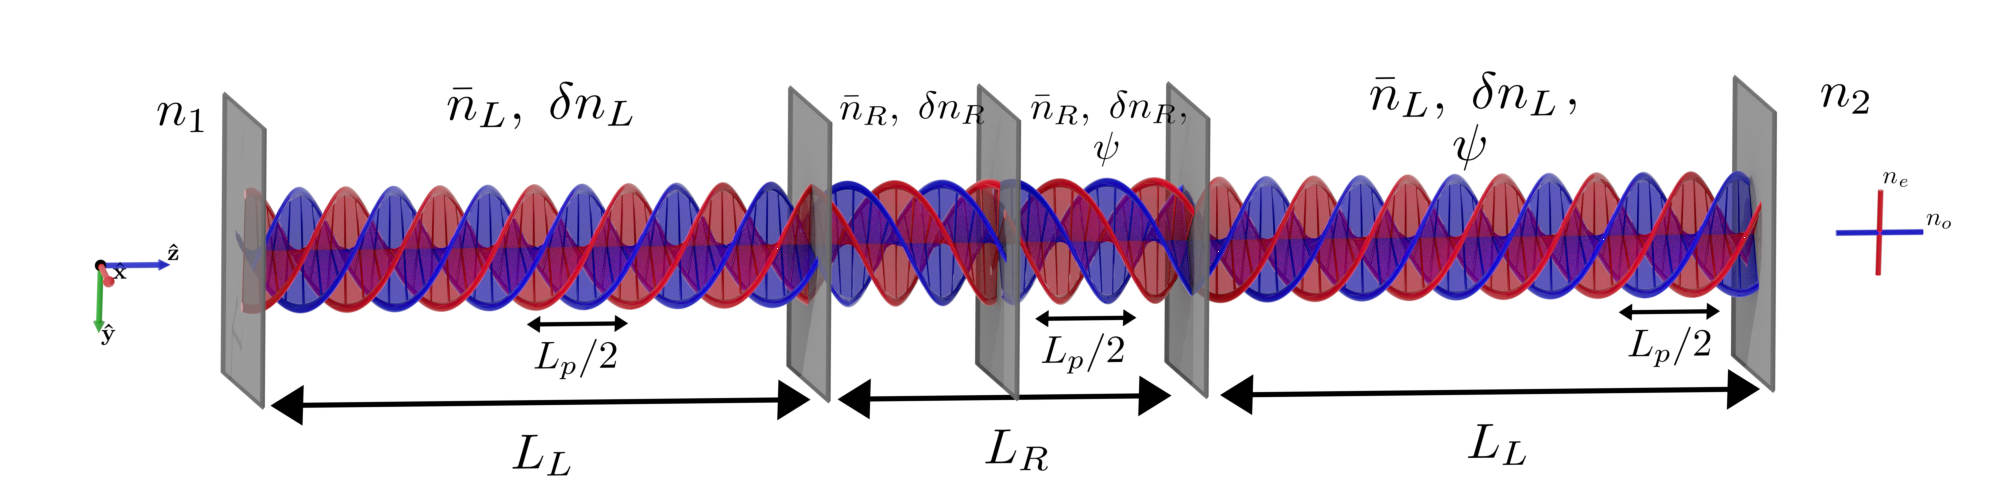
\includegraphics[width=\linewidth]{images/hybrid_defect.png}
		\caption{Hybrid defect cavity}
	\end{figure}
\end{frame}
\begin{frame}{Results : Hybrid defect cavity}
	\begin{figure}
		\begin{subfigure}{0.24\linewidth}
			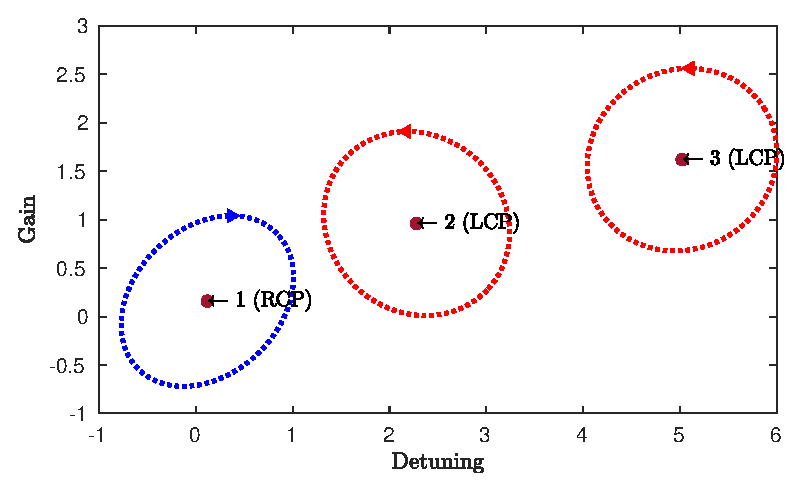
\includegraphics[width=\linewidth]{plots/hybrid_defect/pi_2/modes_found}
			\caption{$\pi/2$ defect}
		\end{subfigure}
		\begin{subfigure}{0.24\linewidth}
			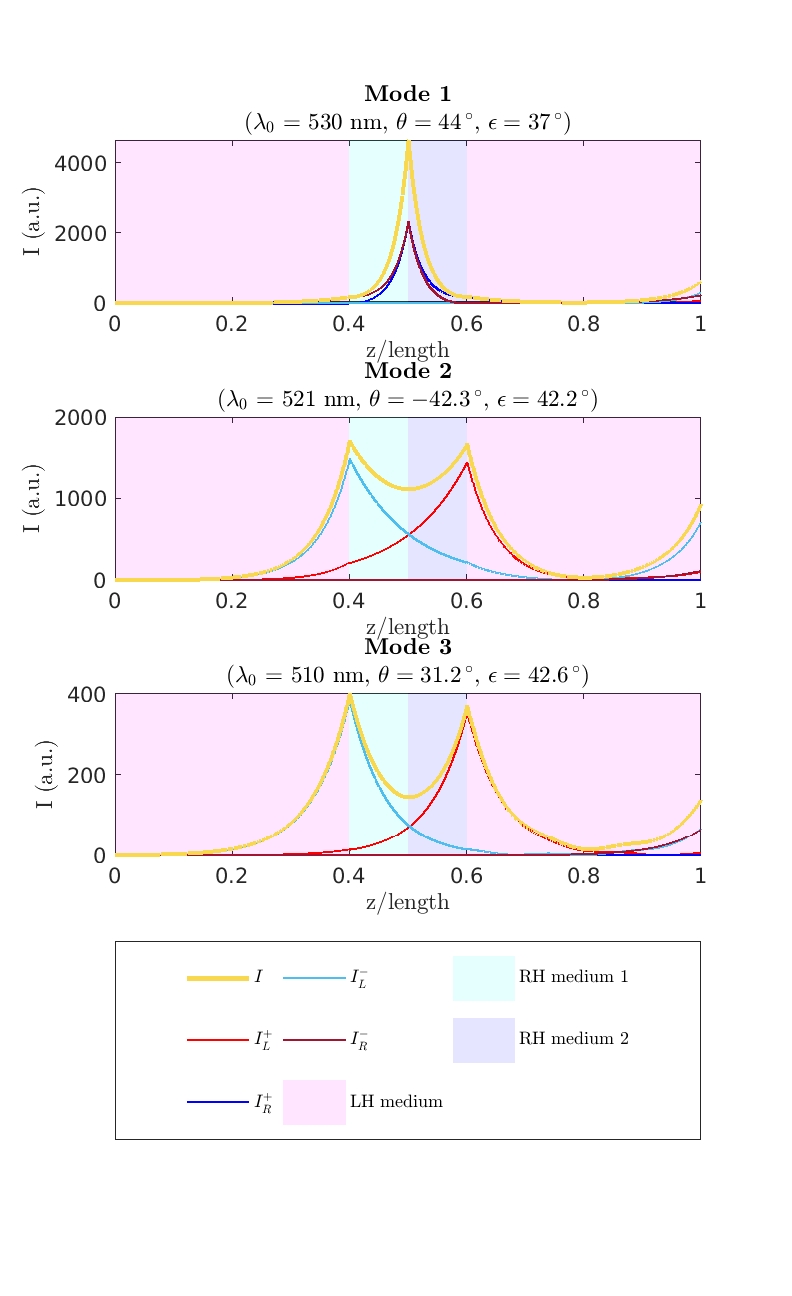
\includegraphics[width=\linewidth]{plots/hybrid_defect/pi_2/intensity_distribution}
			\caption{$\pi/2$ defect}
		\end{subfigure}
		\begin{subfigure}{0.24\linewidth}
			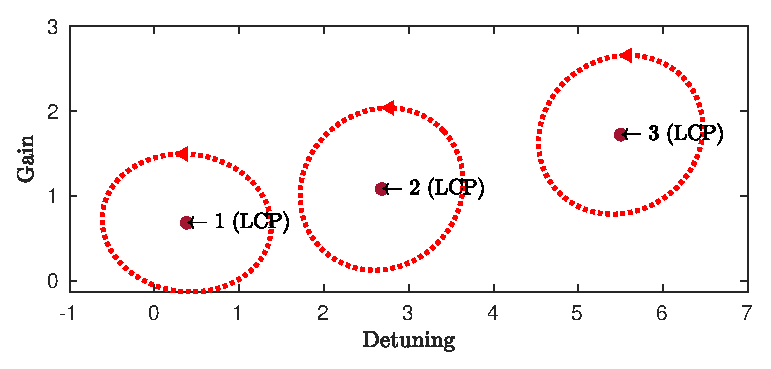
\includegraphics[width=\linewidth]{plots/hybrid_defect/pi_3/modes_found}
			\caption{$\pi/3$ defect}
		\end{subfigure}
		\begin{subfigure}{0.24\linewidth}
			\centering
			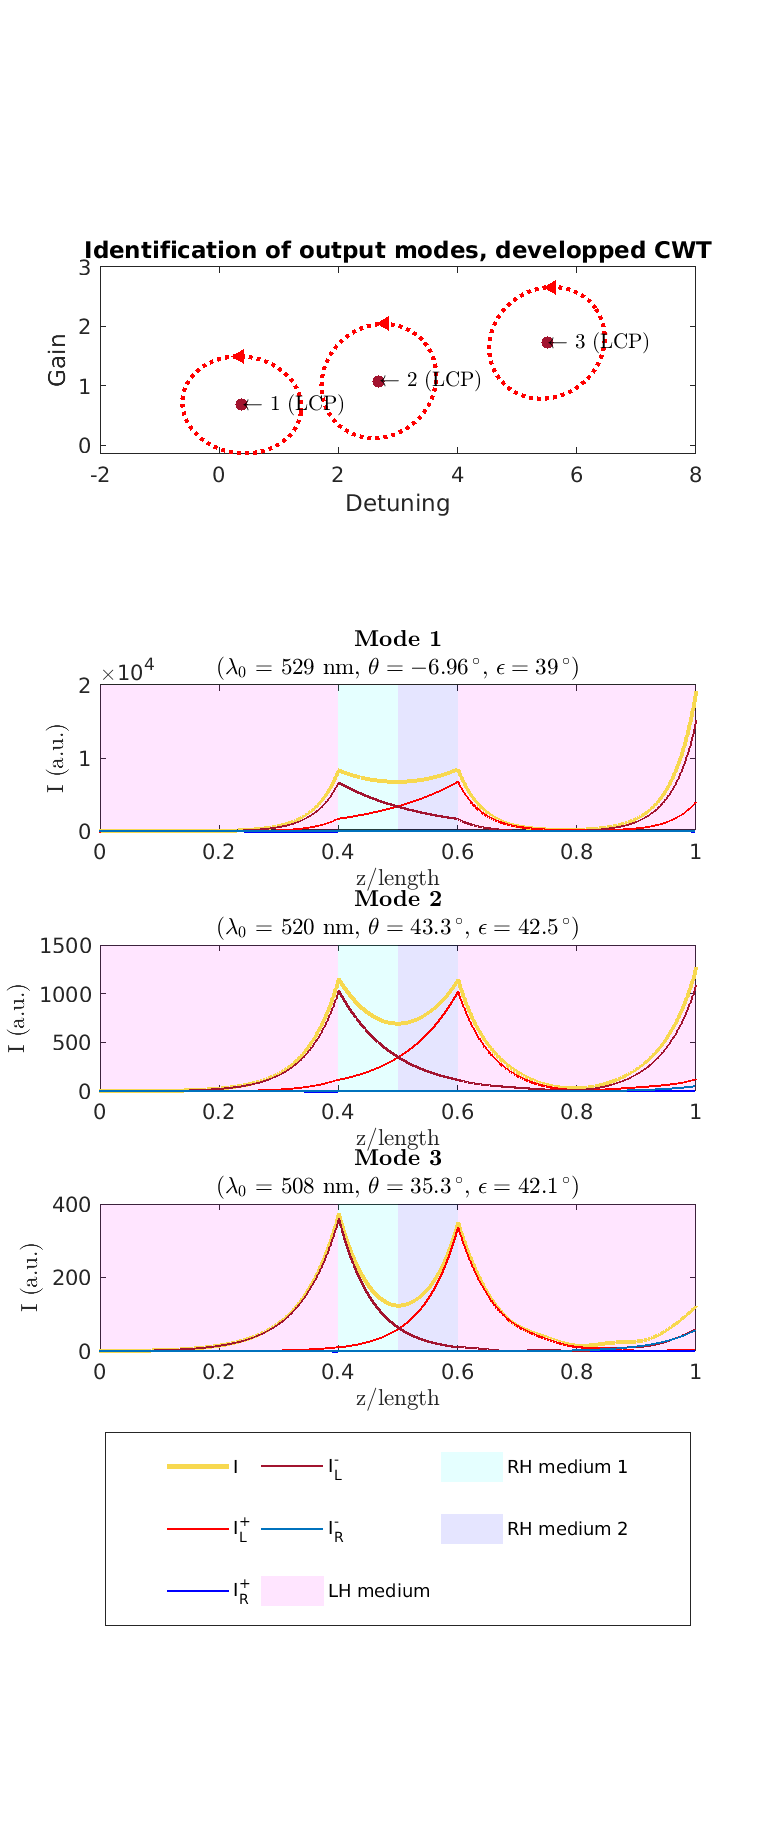
\includegraphics[height=0.8\textheight]{plots/hybrid_defect/pi_3/intensity_distribution}
			\caption{$\pi/3$ defect}
		\end{subfigure}
	\end{figure}
\end{frame}
\begin{frame}{Results : Hybrid defect cavity}
\begin{figure}
	\centering
	\begin{subfigure}{0.49\linewidth}
		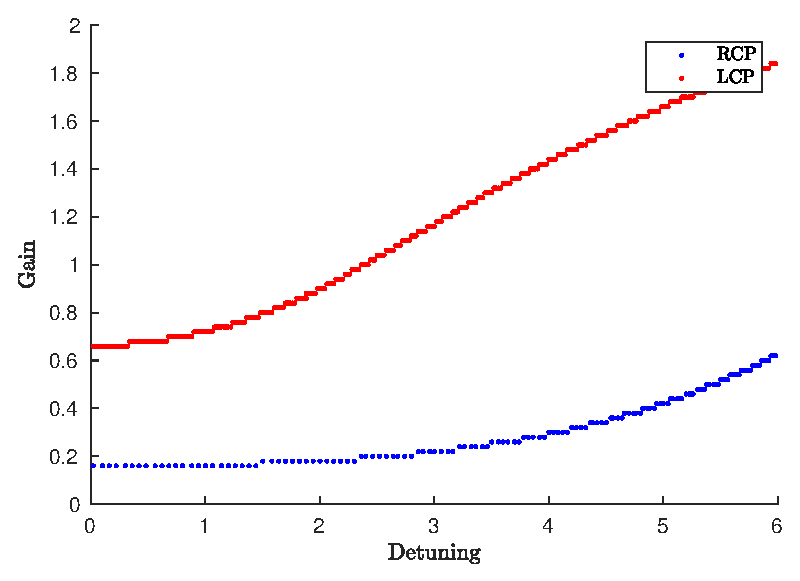
\includegraphics[width=\linewidth]{plots/hybrid_defect/tuning}
	\end{subfigure}
	\begin{subfigure}{0.49\linewidth}
		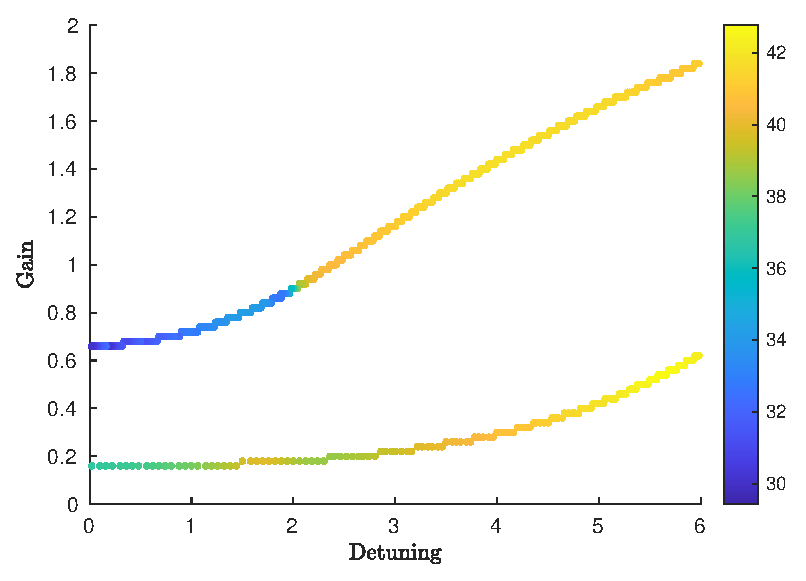
\includegraphics[width=\linewidth]{plots/hybrid_defect/purity_3D}
	\end{subfigure}
\end{figure}
\end{frame}

\begin{frame}{Results : Hybrid defect cavity}
	\begin{figure}
		\centering
		\begin{subfigure}{0.49\linewidth}
			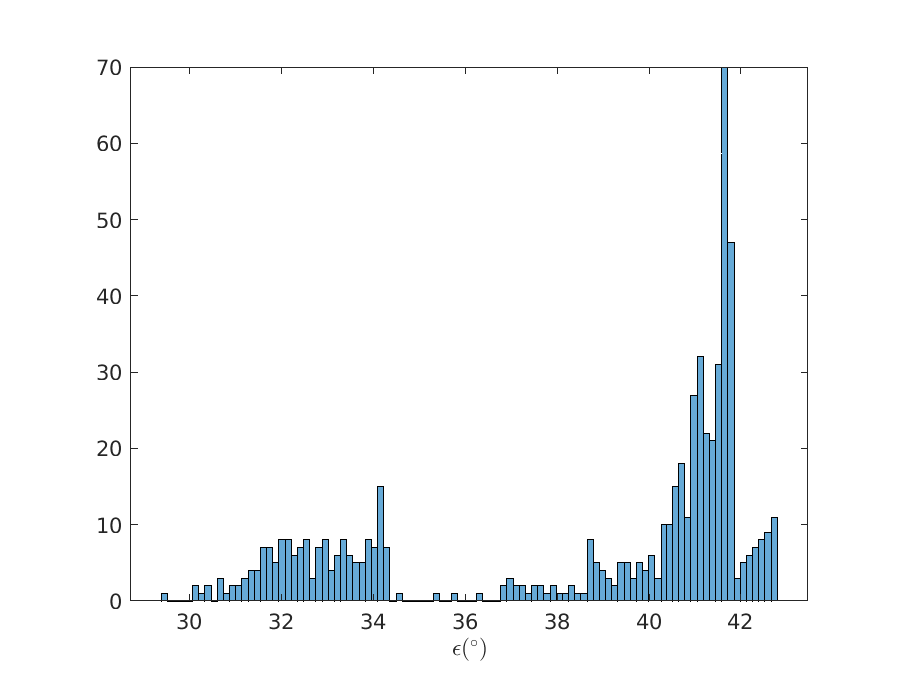
\includegraphics[width=\linewidth]{plots/hybrid_defect/purity}
		\end{subfigure}
		\begin{subfigure}{0.49\linewidth}
			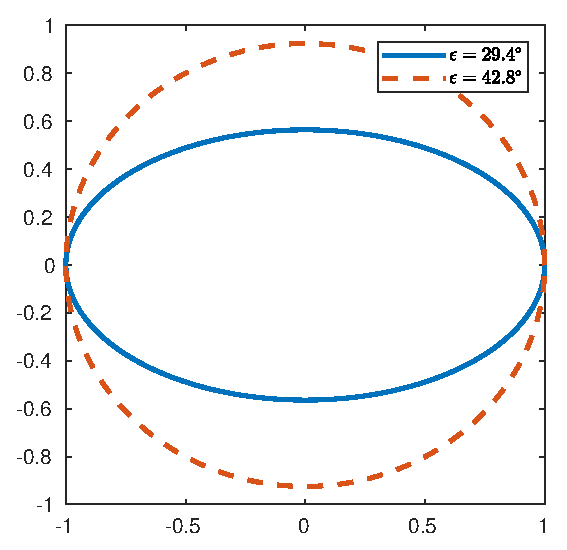
\includegraphics[width=\linewidth]{plots/hybrid_defect/ellipses}
		\end{subfigure}
	\end{figure}
\end{frame}

\section{Conclusion}

\begin{frame}
	\centering
	{\Huge Thank you for your attention !}
	\vfill
	{Do you have any question ?}
\end{frame}

\end{document}